Utilizando como base \textcite{pesquisa}, pode-se dizer que a pesquisa adota
uma abordagem quantitativa e experimental, ou seja, visa analisar e contrastar o desempenho
de diferentes algoritmos em condições controladas. A natureza aplicada do estudo busca não
apenas compreender as nuances de cada algoritmo, mas também oferecer \textit{insights} para a seleção
e implementação dos mais eficazes. A metodologia descritiva permite uma análise detalhada
dos resultados obtidos, destacando as diferenças significativas entre os modelos avaliados.

\section{Solução proposta} \label{sec:solucao}

\begin{figure}[!htb] \centering
    \caption{Fluxo de implementação da solução} \label{figura:proposta}
    \begin{varwidth}{\linewidth}
      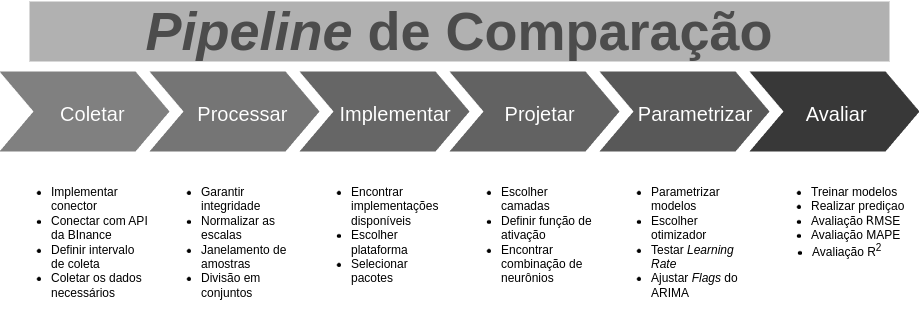
\includegraphics[width=16cm]{figuras/proposta.png}
      \fonte{Elaborado pelo autor, 2024.}
    \end{varwidth}
  \end{figure}

\section{Coleta de dados} \label{sec:coleta}
A coleta de dados, ou obtenção de \textit{Datasets}, envolve inicialmente selecionar locais como APIs, bancos de dados \textit{online} ou arquivos históricos que forneçam os dados em um formato estruturado, como JSON, CSV ou TOML.
No entanto, é possível estabelecer um processo de coleta automatizada através de \textit{Crawlers} ou \textit{Web Scrapping} para extrair as informações brutas.
Independentemente da escolha, sempre é preciso realizar um projeto de dados, que envolve a definição de quais informações são relevantes e sua correlação; para isso, existem métodos como a análise exploratória de dados, do inglês \textit{Exploratory Data Analysis} (EDA).
A Tabela \ref{tab:amostras} contém um exemplo de amostras que foram coletadas, contendo informações de volume, que indicam a intensidade de negociações; trocas, que representam a proporção de compras ou vendas; e preço, que é o valor de fechamento do ativo para aquele \textit{Candle} de quinze minutos.

\section{Pré-processamento} \label{sec:preprocessamento}
No processo de análise de dados, é comum que os dados brutos apresentem inconsistências, como valores ausentes, duplicados ou mal formatados. 
Essas imperfeições comprometem a eficácia dos modelos; por isso, antes de enviar os dados para o treinamento, é crucial assegurar que estejam completos, formatados e escalonados de maneira adequada.
A essa etapa, dá-se o nome de pré-processamento.

\begin{table}[!htb]
    \caption{Amostras da base de dados coletada} \label{tab:amostras}
    \begin{tabularx}{\textwidth}{X|X|X|X}
    \hline
    Data (GMT-3) & Volume (USDT) & Trocas (Total) & Preço (USDT) \\ \hline
    2020-01-01 00:00:00   & 1959651,83      & 2811            & 7228,5         \\ \hline
    2020-01-01 00:15:00   & 1225409,70      & 1897            & 7237,15        \\ \hline
    2020-01-01 00:30:00   & 1469869,68      & 2163            & 7221,27        \\ \hline
    2020-01-01 00:45:00   & 1012436,07      & 1466            & 7225,01        \\ \hline
    2020-01-01 01:00:00   & 1102372,81      & 1985            & 7219,09        \\ \hline
    \end{tabularx}
    \fonte{Elaborado pelo autor, 2024.}
\end{table}

\subsection{Validação de completude} \label{sec:completude}
Para verificar a completude dos dados, foi utilizada uma função nativa do \textit{Pandas}, garantindo que todas as entradas estivessem presentes na base.
Embora o conector a realize na captura, é necessária uma verificação adicional a cada análise para assegurar a qualidade das amostras. 
Caso existam valores ausentes, é possível utilizar métodos como a interpolação linear para estimar os valores faltantes e preenchê-los.

\begin{equation} 
    {P_1(x) = y_0 + \frac{(y_1 - y_0)}{x_1 - x_0} (x - x_0)}
    \label{eq:interpolacao} 
\end{equation}

A interpolação linear (equação \ref{eq:interpolacao}) é baseada na reta que liga dois pontos, na qual \(y_0\) e \(y_1\) são os valores conhecidos para os pontos
\(x_0\) e \(x_1\) entre a variável \(x\), que se deseja calcular o correspondente \(P\).

\subsection{Normalização} \label{sec:normalizar}
Em um \textit{Dataset} multivariado, é comum que os valores estejam em escalas distintas. No caso do \textit{Bitcoin}, o preço e o volume variam em ordens de grandeza superiores ao número absoluto de transações.
Isso se deve à própria natureza da dimensão dos dados; por isso, é necessário padronizar as variáveis para que o modelo não seja enviesado.
Uma das técnicas de normalização mais famosas ajusta as colunas para um intervalo que esteja entre o máximo e o mínimo valor encontrado,  chamada \textit{MinMaxScaller}.
\begin{equation}
    {X_{Scalled} = \frac{X-X_{min}}{X_{max}-X_{min}}}
    \label{eq:scalled}
\end{equation}

Na equação acima, $x$ é o valor original da variável; $X_{min}$ é o valor mínimo encontrado na coluna; $X_{max}$ é o valor máximo.
Ao final, obtém-se o equivalente dimensionado da respectiva linha, ajustado em escala de 0 a 1.

\subsection{Limitações e diferenças entre algoritmos} \label{sec:limitacao}
O processamento de dados em diferentes algoritmos, seja no aprendizado de máquina ou modelagem estatística, requer um dimensionamento de dados contundente às necessidades e limitações de cada método.
Ao utilizar RNAs, é comum que o modelo consiga lidar bem com múltiplas variáveis e forneça um arcabouço robusto de soluções adquiridas durante o treinamento.

Por outro lado, modelos como a regressão linear são tradicionalmente univariados, significando que modelam uma única variável de interesse.
Outra característica é que não são treinados no sentido tradicional; em vez disso, ajustam seus parâmetros diretamente aos valores históricos, requerendo dados estacionários.
Ou seja, as entradas devem ser ligeiramente adaptadas de acordo com a arquitetura.

\subsection{Janelamento} \label{sec:janelamento}

Ao se trabalhar com séries temporais, é comum a separação dos dados em segmentos menores,
 a fim de capturar a dinâmica ao longo do tempo.
Uma dessas técnicas envolve a criação de janelas deslizantes, nas quais um intervalo fixo de observações é utilizado para prever os próximos valores.
No contexto de RNNs, essa abordagem é bastante útil, pois permite que o modelo capture padrões locais e evolutivos, aproveitando o poder da memória da RNA para entender sequências.

Entretanto, quando se trata de modelos estatísticos, o processo de segmentação é, geralmente, feito de maneira incremental.
Em vez de se usar uma janela deslizante de tamanho fixo, o modelo pode se beneficiar de uma janela expansiva, onde todos os dados disponíveis até um determinado ponto são utilizados para fazer a previsão seguinte.
Isso torna justa a comparação, visto que o máximo de informação disponível é utilizado para cada previsão.

\begin{figure}[!htb] \centering
    \caption{Técnicas de janelamento} \label{figura:window}
    \begin{varwidth}{\linewidth}
      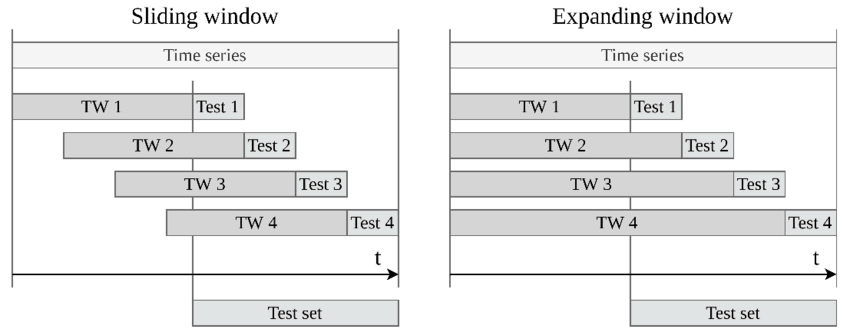
\includegraphics[width=12cm]{figuras/window.png}
      \fonte{\citefonte{Sliding}.}
    \end{varwidth}
\end{figure}
  

\subsection{Divisão em conjuntos} \label{sec:divisao}
Para avaliar a eficácia dos modelos de aprendizado supervisionado, a base de dados é dividida em três subconjuntos: treinamento, validação e teste.
O conjunto de treinamento é usado para ajustar os pesos do modelo, enquanto o de validação serve para otimizar os hiperparâmetros com base na função de perda.
Após o limite de épocas, o conjunto de teste, que contém dados que o modelo ainda não viu, é empregado para verificar a capacidade de generalizar seu desempenho. A etapa não é necessária para o ARIMA, que ajusta seus parâmetros diretamente sobre todos os dados.

\begin{figure}[!htb] \centering
    \caption{Divisão de dados} \label{figura:train_test}
    \begin{varwidth}{\linewidth}
      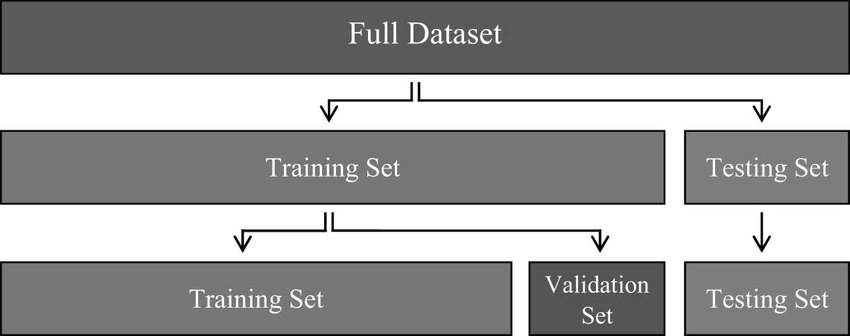
\includegraphics[width=12cm]{figuras/train_test.png}
      \fonte{\citefonte{Sliding}.}
    \end{varwidth}
\end{figure}

\section{Implementação} \label{sec:implementacao}
Todos os modelos foram desenvolvidos utilizando-se a linguagem de programação \textit{Python}, versão 3.10 \cite{ramalho}, juntamente com as bibliotecas \textit{Pandas} e \textit{Numpy} \cite{Data}. 
Na implementação de RNNs, foram utilizados os \textit{Frameworks} Keras 3.10 e TensorFlow 2.10 \cite{maosaobra}. Essas ferramentas podem ser adaptadas para processamento paralelo em GPU, mas, para isso, a placa de vídeo deve ter suporte a CUDA, tecnologia de código aberto da NVIDIA.
O ARIMA foi feito e otimizado com base no Pmdarima, biblioteca que implementa o modelo de forma eficiente.

\section{Arquitetura} \label{sec:arquitetura}
Para \textcite{Good}, a arquitetura de uma RNA define sua estrutura geral, incluindo o número de unidades e a forma como estão conectadas entre si.
Cada modelo foi implementado de acordo com as especificações definidas para avaliação, respeitando as particularidades de cada um em relação à estrutura e aos parâmetros ajustados.
Foram testadas diversas arquiteturas adicionando e removendo camadas, trocando funções de ativação e ajustando o número de neurônios.
Apesar de parecer intuitivo utilizar a arquitetura mais robusta possível, nem sempre é o mais eficiente, visto que sistemas complexos podem sofrer de \textit{overfitting}.
A seguir, são apresentadas as principais características que os diferenciam e justificam seu desempenho nas análises.

\begin{table}[h!] \label{tabela:lstm_struct}
    \caption{Estrutura do modelo baseado em LSTM}
    \begin{tabularx}{\textwidth}{X|X|X|c|X} \hline
    Camada & Tipo & Neurônios & Função de Ativação & Parâmetros \\ \hline
    1 & LSTM                    & 32 & Tangente Hiperbólica                           & 4.000                  \\ \hline
    2 & Densa                   & 32 & Tangente Hiperbólica                            & 1.056                    \\ \hline
    3 & Densa                   & 1  & Linear                           & 33                     \\ \hline
    \end{tabularx}
    \fonte{Elaborado pelo autor, 2024.}
\end{table}

\begin{table}[h!] \label{tabela:gru_struct}
    \caption{Estrutura do modelo baseado em GRU}
    \begin{tabularx}{\textwidth}{X|X|X|c|X} \hline
    Camada & Tipo & Neurônios & Função de Ativação & Parâmetros \\ \hline
    1      & GRU  & 32  & Tangente Hiperbólica     & 3.552                 \\ \hline
    2      & Densa & 32 & Tangente Hiperbólica     & 1.056                    \\ \hline
    3      & Densa & 1  & Linear                   & 33                     \\ \hline
    \end{tabularx}
    \fonte{Elaborado pelo autor, 2024.}
\end{table}

\begin{table}[h!] \label{tabela:bidirectional_struct}
    \caption{Estrutura do modelo baseado em camadas Bidirecionais}
    \begin{tabularx}{\textwidth}{X|X|X|c|X} \hline
    Camada & Tipo & Neurônios & Função de Ativação & Parâmetros \\ \hline
    1                   & Bidirectional            & 32                   & Tangente Hiperbólica                         & 9.216                \\ \hline
    2                   & Densa                   &  32               & Tangente Hiperbólica                           & 2.000                 \\ \hline
    3                   & Densa                   &  1                   & Linear                       & 33                     \\ \hline
    \end{tabularx}
    \fonte{Elaborado pelo autor, 2024.}
\end{table}
    





\section{Configuração} \label{sec:configuracao} 
Os parâmetros das RNAs foram definidos de forma geral e aplicados uniformemente a todos os modelos avaliados.
Utilizar o fator de decaimento aliado ao \textit{Huber} como função de perda é uma estratégia comum, que se mostrou eficaz em garantir a convergência do modelo.
Outros otimizadores, como o \textit{Adam} e o \textit{Adamax}, foram incluídos; todavia, o \textit{Nadam} se mostrou mais eficiente ao atingir o menor erro.
A configuração padrão adotada é descrita detalhadamente na Tabela \ref{tabela:parametros}.

\begin{table}[h!]
    \caption{Configuração dos parâmetros das redes neurais} \label{tabela:parametros}
    \begin{tabularx}{\textwidth}{X|X} \hline
    Parâmetros & Valores \\ \hline
    Batch         & 32               \\ \hline
    Épocas         & 500              \\ \hline
    Otimizador               & Nadam ($\eta=1*10^{-4}$; $\beta_1=0{,}85$; $\beta_2=0{,}989$; $\epsilon= 1*10^{-6}$)             \\ \hline
    Fator de decaimento          & 0,5 em 20 épocas de paciência           \\ \hline
    Função de perda          & Huber              \\ \hline
    \end{tabularx}
    \fonte{Elaborado pelo autor, 2024.}
\end{table}

\section{Avaliação} \label{sec:avaliacao}
Para avaliar a acurácia dos modelos de previsão, foi preciso separá-los em duas categorias: aprendizado de máquina e estatística.
No aprendizado de máquina (supervisionado), é possível validar diretamente na função de perda, que, no caso, é a Huber, enquanto, nos estatísticos, o cálculo é inerente à fórmula.
A escolha da \textit{loss function} se deve à sua capacidade de lidar com \textit{outliers} e ruídos observados principalmente em intervalos curtos, o que se encaixa no contexto de quinze minutos \cite{Jaiswal}.

Na comparação final, efetuou-se uma combinação de métricas estatísticas 
que permitem analisar tanto a precisão quanto a robustez das previsões.
As métricas escolhidas para essa avaliação foram: 
\textit{Root Mean Squared Error} (RMSE), \textit{Mean Absolute Percentage Error (MAPE)} e o Coeficiente de Determinação (R²). Cada uma dessas métricas fornece uma perspectiva única sobre a qualidade das previsões e serão descritas a seguir.

\begin{equation}
Huber = 
\begin{cases} 
\frac{1}{2} a^2, & \text{se } |a| \leq \delta \\
\delta (|a| - \frac{1}{2} \delta), & \text{se } |a| > \delta 
\end{cases}
\label{eq:Huber Loss}
\end{equation}

Na Equação \ref{eq:Huber Loss} acima, \textit{a} representa a diferença entre o valor real $y$ e o valor predito  $\hat{y}$, e o delta ($  \delta $) é um parâmetro que controla o ponto de transição entre os dois regimes de penalização (quadrática e linear). Para erros pequenos, a perda é quadrática, enquanto, para erros grandes, a perda se apresenta linear, o que torna a função robusta a \textit{outliers}.

\begin{equation}
    \text{RMSE} = \sqrt{\frac{1}{n} \sum_{t=1}^{n} (y_t - \hat{y}_t)^2}
    \label{eq:rmse}
\end{equation}

A principal métrica descrita na Equação \ref{eq:rmse} é medir a diferença entre os valores observados 
y e os valores preditos $\hat{y}$, elevando o erro ao quadrado antes de se calcular a média e aplicando a raiz quadrada ao final, para que o erro tenha a mesma unidade dos dados originais. Isso significa que o RMSE dá maior peso a erros maiores devido ao efeito do quadrado.

\begin{equation}
    \text{MAPE} = \frac{1}{n} \sum_{t=1}^{n} \left|\frac{y_t - \hat{y}_t}{y_t}\right|
    \label{eq:mape}
\end{equation}

A Equação \ref{eq:mape} é média dos erros percentuais absolutos na série, padronizando a análise para que seja possível comparar diferentes escalas ou unidades.
Quando a diferença entre y e ŷ é dividida por y, obtém-se o percentual, que é, então, normalizado pela média. Como o somatório de valores decimais pode ser confuso, alguns autores sugerem multiplicar cada resultado por 100, para facilitar a interpretação.

\begin{equation}
    R^2 = 1 - \frac{\sum_{t=1}^{n} (y_t - \hat{y}_t)^2}{\sum_{t=1}^{n}(y_t - \bar{y})^2}
    \label{eq:r2}
\end{equation}

O erro $R^2$ (equação \ref{eq:r2}), também chamado de coeficiente de determinação, representa a proporção da variabilidade dos dados, que é explicada pelo modelo, variando de 0 a 1, sendo 1 o ajuste perfeito.
O $y_t$ define os valores reais; $\hat{y}_t$, os valores preditos; e $\bar{y}$, a média dos valores observados. O numerador contém a soma dos erros ao quadrado entre os valores reais e preditos (erro do modelo), enquanto o denominador é a soma da variabilidade total dos dados.

\section{Materiais e Tecnologias} \label{sec:materiais}
Para a realização deste trabalho, 
foram utilizados um processador Intel Core i5-12500H e
uma placa de vídeo NVIDIA GeForce RTX 3050 de 4GB com suporte a CUDA 12.
Um total de 16 GB de memória RAM foram utilizados para armazenar os tensores, parâmetros e janelamento em memória dos dados. 
O sistema operacional foi o Linux Pop! OS 20.04, e o desenvolvimento foi feito no editor Visual Studio Code, utilizando Python 3.10. As bibliotecas empregadas incluíram Pandas e Numpy, para manipulação e computação de dados, e Matplotlib e Seaborn, para visualização. Para aprendizado de máquina e RNNs, empregaram-se os frameworks Keras e TensorFlow, e o modelo ARIMA foi implementado com a biblioteca Pmdarima.